%%%%%%%%%%%%LASCIARE QUESTI COMMENTI!!!%%%%%%%%%%%%%%%%
% !TeX document-id = {02478c5b-a4cd-4f4c-a426-82311f1967ba}
% !TeX TXS-program:compile = txs:///pdflatex/[--shell-escape]
%%%%%%%%%%%%%%%%%%%%%%%%%%%%%%%%%%%%%%%%%%%%%

\documentclass[10pt,hidelinks]{article}
\usepackage[utf8]{inputenc}
\usepackage[british]{babel}
\usepackage{mdframed}

%%MUST STAY HERE
\usepackage[svgnames, table]{xcolor}
%%

\usepackage{algorithm}
\usepackage{algpseudocode}
\usepackage{amsfonts}
\usepackage{amsthm}
\usepackage{amsmath}
\usepackage{array}
\usepackage{amssymb}
\usepackage{arydshln}

\usepackage{bbding}
\usepackage{booktabs}

\usepackage[colorlinks = true,
            linkcolor = pdarkerblue,
            urlcolor  = gblue,
            citecolor = gblue,
            anchorcolor = blue]{hyperref}%%Must stay here
%%

\usepackage{calc}
\usepackage[labelfont={bf,sf,footnotesize,color=pblue},textfont={footnotesize}, margin={40pt,40pt}]{caption}
\usepackage{cleveref}
\usepackage{csquotes}
\usepackage{dsfont}

\usepackage{eurosym}

\usepackage{fancyhdr}
\pagestyle{fancy}
\fancyhead{}
\fancyhead[R]{\color{pblue} \sc \nomefico}
\lhead{
\includegraphics[width=1cm]{pics/Cherubino.jpg}}
\usepackage[T1]{fontenc}
\usepackage{fullpage}

\usepackage{geometry}

\usepackage{graphicx}

\usepackage{hhline}
\usepackage{listings}
\usepackage{lipsum}

\usepackage{mathrsfs}
\usepackage{mathtools}
\usepackage{minted}
\usepackage{multicol}
\usepackage{multirow}

\usepackage[numbers,sort]{natbib}
\usepackage{navigator}

\usepackage{palatino}
\usepackage{pifont}
\usepackage{pgffor}
\usepackage{pgfplots}
\usepackage{pgfplotstable}
\usepackage{placeins}

%\usepackage{showframe}
\usepackage{sectsty}
\usepackage{siunitx}
%\usepackage{subfig}
\usepackage{subcaption}

\usepackage{tabularx}
\usepackage[many]{tcolorbox}
\usepackage{tikz}
\usepackage{todonotes}

\usepackage{verbatim}

\usepackage{wrapfig}

\usepackage{xinttools}

%%%~~~~~~~~~~~~~~~~~~~~~~~~Fonts~~~~~~~~~~~~~~~~~~~~~~~%%%


%%%~~~~~~~~~~~~~~~~~~~~~~~~Colours~~~~~~~~~~~~~~~~~~~~~%%%
\definecolor{gblue}{HTML}{000099}
\definecolor{pblue}{HTML}{00004d}%{0000FF}
\definecolor{pdarkblue}{HTML}{000080}
\definecolor{pdarkerblue}{HTML}{000066}
%\definecolor{veryblue}{HTML}{00004d}

%~~~~~~~~~~~~~~~~~~~~~~~~~~~~~Tikz~~~~~~~~~~~~~~~~~~~~~~~~~~~~~%
\usetikzlibrary{calc}
\usetikzlibrary{shapes,arrows,arrows.meta}
\usetikzlibrary{automata,positioning}
\usetikzlibrary{spy,backgrounds}
\usetikzlibrary{matrix,positioning,arrows.meta,arrows}
\usetikzlibrary{fadings}
\usetikzlibrary{positioning}
\usetikzlibrary{fit}

\newcommand{\nomefico}{\textbf{nomeFicoDaScegliere}}
\newcommand{\github}{\texttt{https://github.com/magemma/question-answering}}
\newcommand{\app}{\texttt{https://link-alla-app}}

\pgfplotsset{compat=1.15}

\sectionfont{\bf \Large \color{pblue}}
\subsectionfont{\bf \color{pdarkblue}}
\subsubsectionfont{\bf \color{pdarkerblue}}

\mdfdefinestyle{MyFrame}{%
    linecolor=pdarkblue,
    fontcolor=white,
    outerlinewidth=2pt,
    roundcorner=20pt,
    innertopmargin=4pt,
    innerbottommargin=4pt,
    innerrightmargin=4pt,
    innerleftmargin=4pt,
    leftmargin = 4pt,
    rightmargin = 4pt,
    backgroundcolor=pdarkerblue
}

 \renewcommand{\labelitemi}{$\textcolor{pblue}{\diamond}$}

\DeclareMathOperator*{\avg}{avg}


\def\colOne{white}
\def\colTwo{pblue!10}
\def\colHea{pblue!35}


%%%%%%%%%%%%%%%%%%%%%%%%%%%%%%%%%%%%%%%%%%%%%%%%%%%%%%%%%%%%%%%%%%%%%%%%%%%%%%%%%%

\begin{document}

\begin{mdframed}[style=MyFrame,nobreak=true,align=center,userdefinedwidth=30em]
\textbf{Osservazioni}

\begin{itemize}
    \item I retangoli che vedete ai bordi servono per vedere quanto sono grandi i margini scrivibili della pagina, si possono togliere commentando la riga \texttt{\textbackslash usepackage\{showframe\}}
    \item L'abstract adesso conta 267 parole. Di solito gli abstract non sono piu' lunghi di 300
    \item Il nome del nostro strumento di QA sta in una macro, per usarlo nel report scrivere \texttt{\textbackslash nomefico}
    \item Il link al repo github sta in una macro, per usarlo scrivere \texttt{\textbackslash github}
    \item Il link alla pagina web per QA (ancora da definire) sta in una macro, chiamata \texttt{\textbackslash app}
    \item le immagini sono solo una bozza, vorrei che fossero approvate al 100\% prima di realizzarle in latex
    \item Ho truccato il json di emepio (che e' in questa cartella in formato \texttt{.jsonl}), perche' aveva 36 long answer candidates e non veniva bene l'immagine del json. Se si decide di cambiare esempio, cambiarlo coerentemente
\end{itemize}
\end{mdframed}

\newpage

\begin{titlepage}
    \centering
    \scalebox{0.7} {
        \begin{minipage}{0.22\textwidth}%
            
\includegraphics[width=\linewidth]{pics/Cherubino.jpg}
        \end{minipage}\hspace{10pt}
        \begin{minipage}{0.9\textwidth}%
            \flushright
            \large
            \vspace{0.8cm}
            \textsc{\color{pblue}%
            \nomefico\\
            a Bert-based, open domain\\
            question answering system}
            
\begin{tikzpicture}%
                \draw[thick, brown] (0.1,0)--(0.99\textwidth,0);%   
            \end{tikzpicture}%
        \end{minipage}%
    }

    \vspace{0.3cm}
    
    Gabriele Barreca, Mario Bonsembiante {\small and} Gemma Martini
    
    %\vspace{0.4cm}
    
    {\scriptsize University of Pisa}
    
    \vspace{0.2cm}
    
    \abstract{
    \scriptsize
    Question answering (QA) systems can be seen as information retrieval systems which aim is to respond to queries, stated in natural language, by returning short answers or long sentences.
    The ``so-called'' \emph{open domain QA task} adds the challenge of understanding if the answer to the selected question may or may not be found in a given paragraph, which content has been buried within large text corpora, such as Wikipedia.

    \vspace{0.1cm}

    Building such systems for practical applications has historically been quite challenging and involved.
    The spectrum of possible answers given a question and a paragraph, moves from the ``simple'' \emph{yes/no answers} to the longer and more articulated \emph{long answers}, to then get to a trade-off between expressive power and succinctness, the ``so-called'' \emph{short answers}, which aim to enclose the answer in a single and possibly short sentence.
    
    \vspace{0.1cm}
    
    In this paper, we present a BERT-based implementation that solves an open domain QA task, providing all the three categories of answers listed above, with particular attention on the most widely studied kind, i.e.~short answers.
    We achieve pretty good results, although not as good as the state-of-the-art, that was not the purpose of this work.

    
    As expected and already stated in previous work, we conclude that predicting long answers per se is pretty unreliable, while much better results are achieved if the short answer is predicted and then enlarged with the whole paragraph it lies in, from the original text.
}
    
    \vspace{1cm}
    
    
\begin{tikzpicture}%
        \draw[thick, brown] (0,0)--(0.8\textwidth,0);%   
    \end{tikzpicture}%
    
    %\vspace{-0.5cm}
    \scalebox{0.8}{\vbox{\tableofcontents}}
    %\tableofcontents

    \vspace{0.3cm}

    
\begin{tikzpicture}%    
        \draw[thick, brown] (0,0)--(0.8\textwidth,0);%   
    \end{tikzpicture}%

    %{\large \today}
    \vfill
\end{titlepage}

%%%%%%%%%%%%%%%%%%%%%%%%%%%%%%%%%%%%%%%%%%%%%%%%%%%%%%%%%%%%%%%%%%

%\thispagestyle{empty}
\newpage
\newgeometry{
	right=45mm,
	left=40mm,
	top=40mm,
	bottom=45mm
}
\setcounter{page}{1}

%%%%%%%%%%%%%%%%%%%%%%%%%%%%%%%%%%%%%%%%%%%%%%%%%%%%%%%%%%%%%%%%%%
\section{Introduction}\label{sec:intro}
%%%%%%%%%%%%%%%%%%%%%%%%%%%%%%%%%%%%%%%%%%%%%%%%%%%%%%%%%%%%%%%%%%

\todo[inline]{Aggiungere introduzione}
\todo[inline]{aggiungere una frase in cui si dice che cosa si trova in quali sezioni}


%%%%%%%%%%%%%%%%%%%%%%%%%%%%%%%%%%%%%%%%%%%%%%%%%%%%%%%%%%%%%%%%%%
\section{The architecture}\label{sec:model}
%%%%%%%%%%%%%%%%%%%%%%%%%%%%%%%%%%%%%%%%%%%%%%%%%%%%%%%%%%%%%%%%%%
Before digging into the details of the machine learning core of our BERT-based QA system, let us define the outline of the responsive QA tool we developed.

In \Cref{fig:tool_dataflow} there is a pictorial representation of how the user interacts with the system, how it processes the information (server side) and how it prompts the results.

\begin{figure}[ht!]
    \centering
    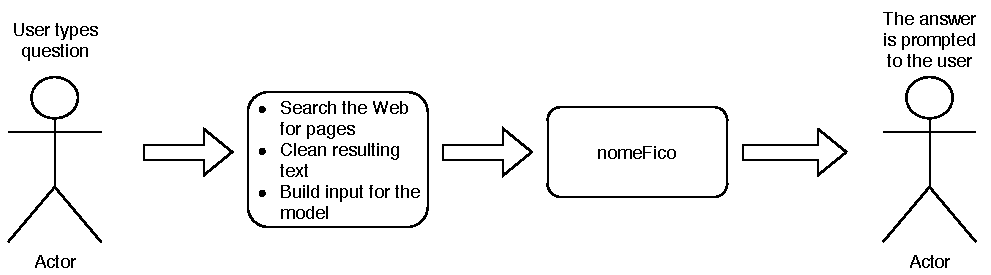
\includegraphics[width=0.9\textwidth]{pics/tool_dataflow.pdf}
    \caption{The full functioning of \nomefico, combined with an effective user interface.}\label{fig:tool_dataflow}
\end{figure}

\todo[inline]{Aggiungere descrizione con immagini del workflow dell'applicazione, con un esempio che funziona, magari creando una sottosezione.}

\subsection{\nomefico}\label{subsec:nomefico}
We are now ready to discuss the implementation of \nomefico.

We decided to tackle the open domain QA task by creating a stack of two neural networks, forming a two-layer architecture, as shown in \Cref{fig:broad_architecture}.

\begin{figure}[ht!]
    \centering
    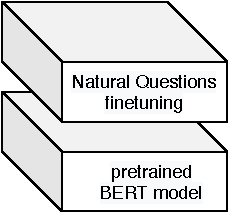
\includegraphics[width=0.3\textwidth]{pics/broad_architecture.pdf}
    \caption{Sketch of the architecture of \nomefico.}\label{fig:broad_architecture}
\end{figure}

The first layer is built using BERT's~\cite{devlin2018bert} checkpoints~\footnote{In practice, we run experiments using also ALBERT~\cite{albert} and BERT Large. In the future also RoBERTa's~\cite{roberta} checkpoints will be used.} from Hugging Face, while the second layer is a neural network that uses BERT's embeddings and the Natural Questions (NQ)~\cite{kwiatowski} dataset~\footnote{Some qualities of NQ are the following: (1) the questions were formulated by people out of genuine curiosity or out of need for an answer to complete another task, (2) the questions were formulated by people before they had seen the document that might contain the answer, (3) the documents in which the answer is to be found are much longer than the documents used in some of the existing question answering challenges.} with the aim of obtaining the answer to the question.

In the following paragraphs, the reader can find a more detailed explanation of the two layers.

\subsubsection{BERT}\label{subsubsec:bert}
Bidirectional Encoder Representations from Transformers (BERT)~\cite{devlin2018bert}  has been introduced by Google in 2018 and it has been defined as the biggest leap forward in the past five years.

Let us dig into details a bit more and explain how the BERT layer works.

BERT is an embedder, i.e.~a neural network that translates words (more generally sentences and whole paragraphs) into sets of $512$-dimensional vectors\todo{siamo sicuri sul 512?}.
One of the main advantages introduced by this technology is the way BERT splits words into tokens (tokenization process): it allows to split words into smaller pieces, before mapping them into vectors.
This choice has the advantage of allowing the encoding of words that are not present in the dictionary and to represent all the words that share a prefix using a root vector and different representations for suffixes.

The second and more crucial advantage introduced by BERT is the bidirectional self attention mechanism, that takes into account not only all the words that precede the target word, but also the rightmost part, giving to every word a context.




\todo[inline]{Fare digressione sull'utilizzo di BERT o BERT-large o ALBERT}

As a recap, BERT (or BERT-based models) provides word-piece tokenization, a masked language model and  the ``next sentence'' prediction, but it needs to be fine-tuned for a specific task, such as QA.

\subsubsection{Fine-tuning}\label{subsubsec:finetuning}
In this work the authors decided to fine tune the model on Natural Questions dataset.

Each training pattern is a \texttt{json} object, it is stored in a line and it has the following structure (see \Cref{fig:json}):

\begin{figure}[ht!]
	\centering
	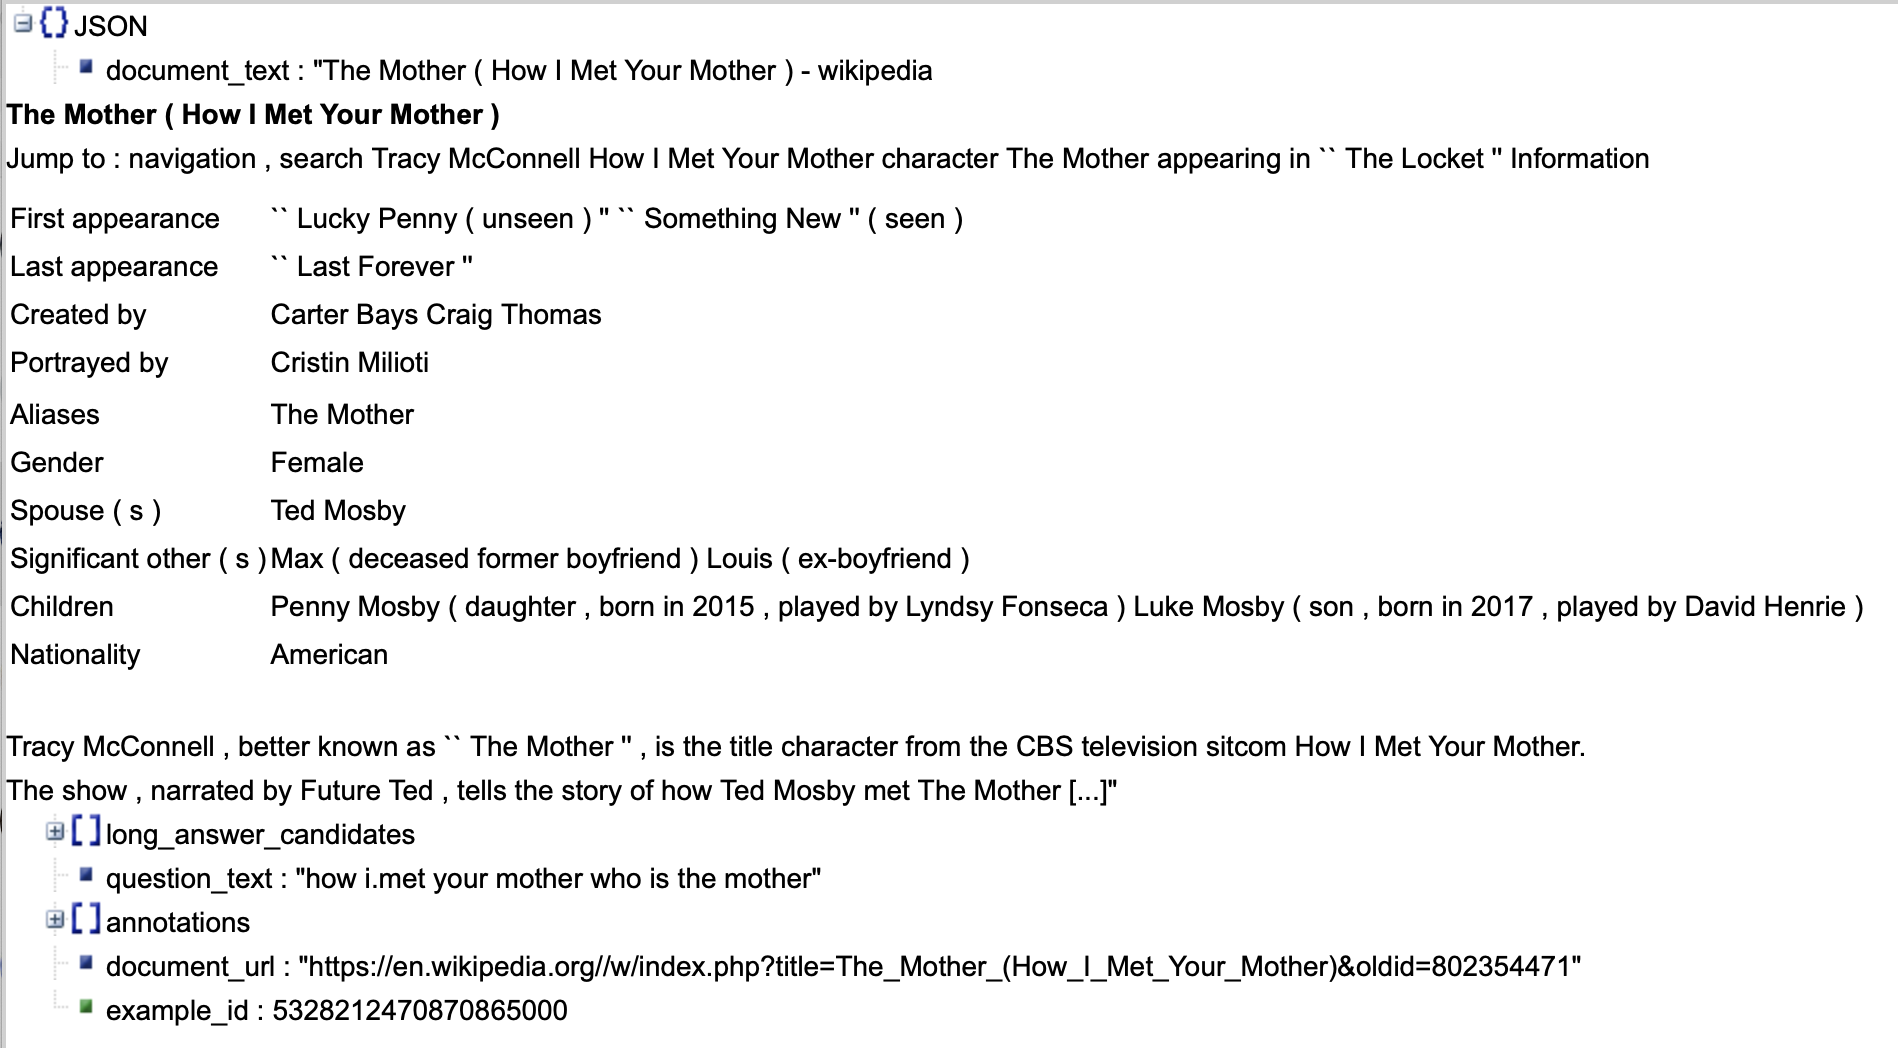
\includegraphics[width=0.8\textwidth]{pics/json.png}
	\caption{Broad structure of an input pattern.}\label{fig:json}
\end{figure}

\begin{itemize}
	\item {\tt document\_text}: the HTML (cleaned of some tags) of the paragraph that may contain the answer;
	\item {\tt long\_answer candidates}: contains the original question and a list of start and end positions of candidates for the answer (an example in \Cref{fig:long_answer_candidates});
	\item {\tt annotations}: contains three sub-objects, that represent if the question allows a ``yes-no'' answer, the information about the short answer and the information about the long answer respectively (as shown in \Cref{fig:annotations}). It is possible that a question does not allow to be answered looking at the paragraph given as input. In that case the fields in the \texttt{long\_answer} object have value $-1$ and the list \texttt{short\_answers} is empty.
\end{itemize}

\begin{figure}[ht]
	\begin{subfigure}{.47\textwidth}
		\centering
		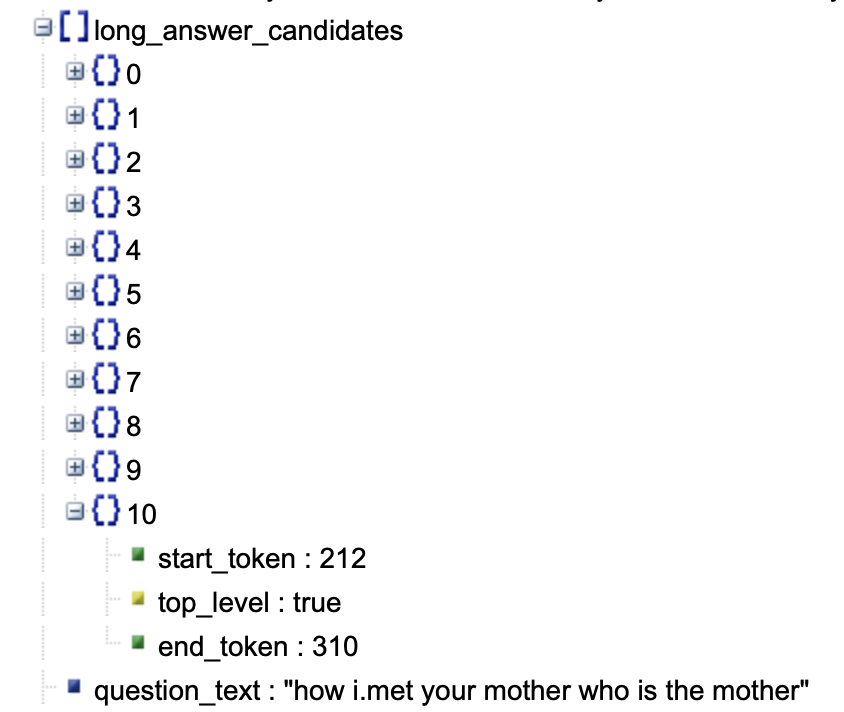
\includegraphics[width=0.95\textwidth]{pics/long_answer_candidates.png}
		\caption{\texttt{long\_answer candidates}.}\label{fig:long_answer_candidates}
	\end{subfigure}
	\begin{subfigure}{.53\textwidth}
		\centering
		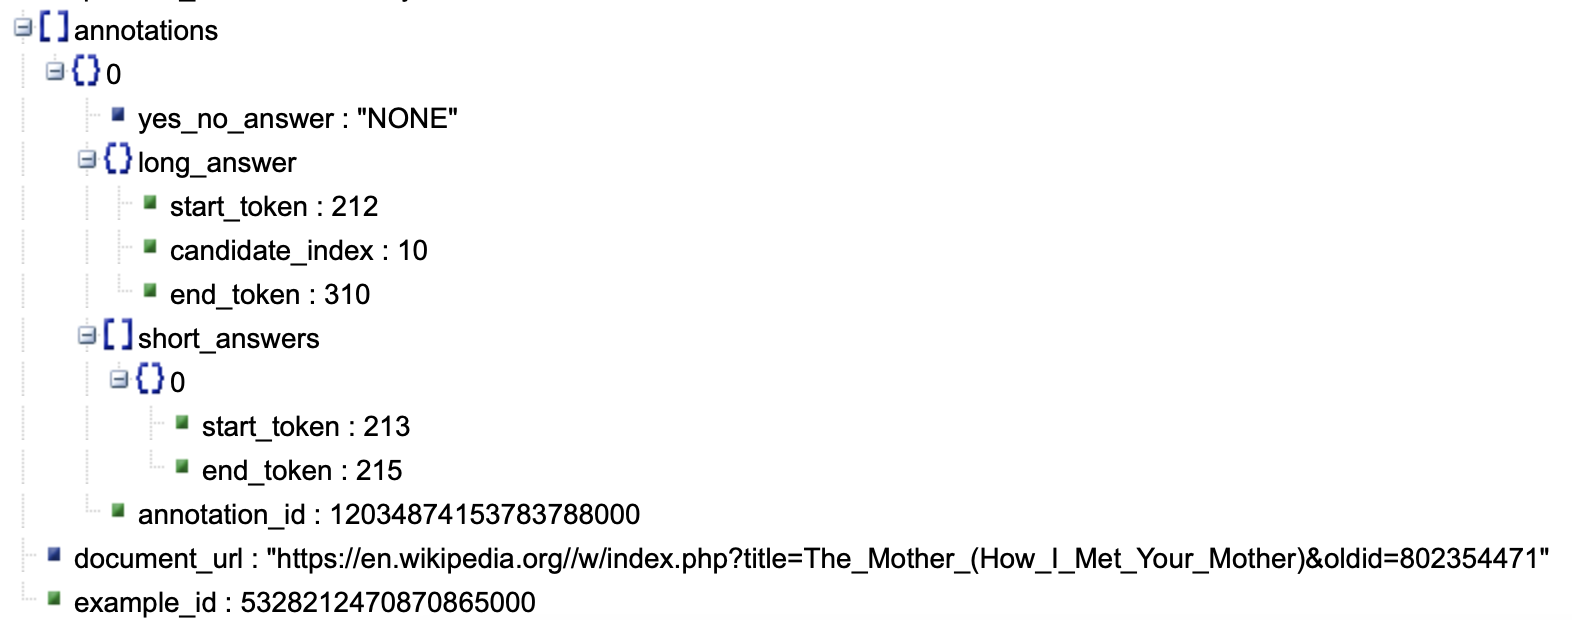
\includegraphics[width=0.95\textwidth]{pics/annotations.png}
		\caption{\texttt{annotations}.}\label{fig:annotations}
	\end{subfigure}
	\caption{More details about the fields of an input pattern.}
	\label{fig:json_zoomed}
\end{figure}

The NQ training set has on average, input patterns with size of $10$MB and the whole training set is stored in a \texttt{.jsonl} file of size $\approx 17$ GB.
It goes without saying that loading both BERT's checkpoints and such file into RAM is not possible, so we managed to overcome this problem by splitting the file into chunks with size smaller than $100$MB.

Another crucial characteristic of this dataset is that is strongly unbalanced towards the questions that are unanswerable:
\blockquote{\it In total, annotators identify a long answer for $49\%$ of the examples, and short answer spans or a yes/no answer for $36\%$ of the examples. We consider the choice of whether or not to answer a question a core part of the question answering task, and do not discard the remaining $51\%$ that have no answer labeled.\cite{kwiatowski}}
	
This issue of unbalanced data needs some more reasoning: as already discussed in \Cref{subsubsec:bert}, the BERT-based embedder maps the input text into vectors. It also performs another operation, namely it splits the paragraph in the so-called ``crops'', containing $512$ tokens.
It is easy to conclude that most of these crops do not contain the answer to the original question, hence the umbalancing becomes even more severe ($\approx 95\%$ of the crops do not contain the answer).

The authors overcame this issue by selecting only the $3\%$ of the so-called ``impossible questions''\footnote{The code is available on GitHub, we set the value $0.03$ to the parameter called \texttt{p\_kepp\_impossible} in \texttt{dataset\_utils\_version2.py}.} and by designing an effective yet simple loss function.

\todo[inline]{Rifare figura}

On a batch of examples, we computed the loss as follows:
\[
\begin{cases}
\frac{\frac{\biggl ( \avg\limits_{\text{batch}} \text{start\_loss} + \avg\limits_{\text{batch}} \text{end\_loss}  \biggr )}{2} + \avg\limits_{\text{batch}} \text{long\_loss}}{2} \hspace{0.5cm}\text{if answerable}\\
0 \hspace{5.3cm} \text{otherwise}
\end{cases}
\]
 
 where *\_loss is the categorical cross-entropy between the position of the true answer and the position of the guess, as shown in \Cref{fig:loss}.

\begin{figure}[ht!]
	\centering
	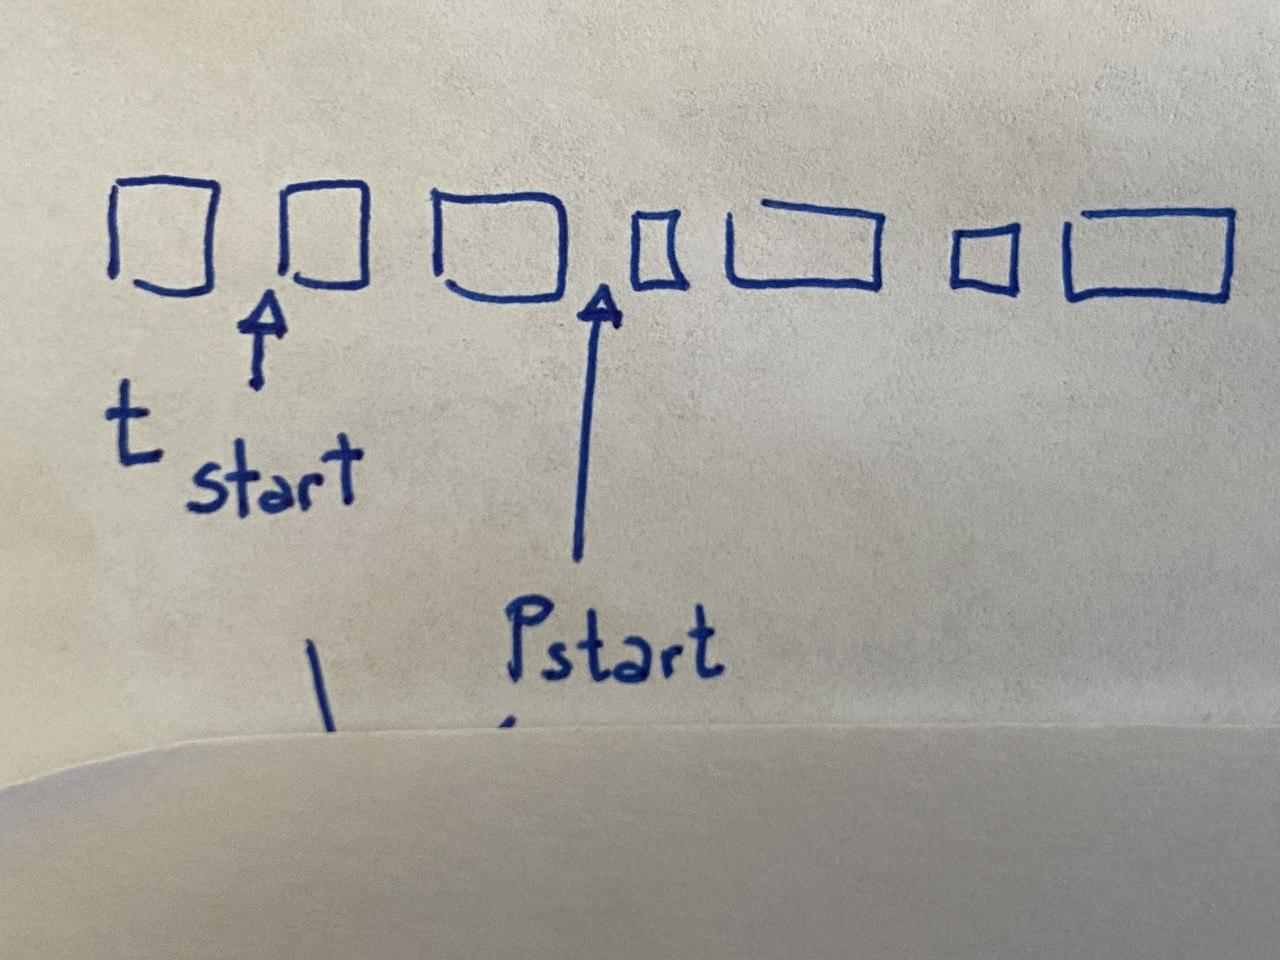
\includegraphics[width=0.4\textwidth]{pics/loss.jpg}
	\caption{A pictorial representation of how the position of the first token of the answer may vary between target and predicted value.}\label{fig:loss}
\end{figure}

\todo[inline]{Scrivere cosa dei token aggiunti \texttt{    tags = ['Dd', 'Dl', 'Dt', 'H1', 'H2', 'H3', 'Li', 'Ol', 'P', 'Table', 'Td', 'Th', 'Tr', 'Ul']}}

%%%%%%%%%%%%%%%%%%%%%%%%%%%%%%%%%%%%%%%%%%%%%%%%%%%%%%%%%%%%%%%%%%
\section{Experimental results}\label{sec:experimental_results}
%%%%%%%%%%%%%%%%%%%%%%%%%%%%%%%%%%%%%%%%%%%%%%%%%%%%%%%%%%%%%%%%%%


%%%%%%%%%~~~~~~~~~~~~~~~~~~~~~~~~~~%%%%%%%%%%
\subsection{Hardware}
%%%%%%%%%~~~~~~~~~~~~~~~~~~~~~~~~~~%%%%%%%%%%


%%%%%%%%%~~~~~~~~~~~~~~~~~~~~~~~~~~%%%%%%%%%%
\subsection{Hyper-parameters values}
%%%%%%%%%~~~~~~~~~~~~~~~~~~~~~~~~~~%%%%%%%%%%

\begin{table}[ht!]
	\footnotesize\centering
	\rowcolors{2}{\colOne}{\colTwo}
	\begin{tabular}{|l|p{60mm}|}
		%HEADER
		\hline\rowcolor{\colHea} Parameter & Values\\\hline\hline
		$ \eta $ (``learning rate'') & $ 1e-4$, $1e-5$, $1e-6$ \\
		$\beta_1$ & $0.9$\\
		$\beta_2$ & $0.999$\\
		$\varepsilon$ & $1e-7$\\
		batch size & $8$ (ALBERT), $4$ (BERT)\\
		\end{tabular}
	\caption{Hyperparameters values.}\label{tab:gridSearchParamCl}
\end{table}


%%%%%%%%%%%%%%%%%%%%%%%%%%%%%%%%%%%%%%%%%%%%%%%%%%%%%%%%%%%%%%%%
\section{Conclusions and future work}\label{sec:conclusions_and_future_work}
%%%%%%%%%%%%%%%%%%%%%%%%%%%%%%%%%%%%%%%%%%%%%%%%%%%%%%%%%%%%%%%%
We describe \nomefico as an interactive question answering platform that sees its application in various contexts, such as domotics or education.
We performed experimental results and validations techniques that assess the goodness of this model, although we highlight some issues that could be solved more effectively in the future, such as the problem of the presence of a typo in the query (both human error in typing or machine speech-to-text misunderstanding)\footnote{One could try to use library already implemented in Python for auto-correction, such as \texttt{auto-correct} available on Pypy, or a more involved and more accurate dictionary-based auto-correct strategy.}.
Moreover, we would like to stress that choosing to force the model to learn only the answerable question was only a first approach to solve the problem and that another technique worth deepening in the future may be using a binary classification layer to check if the answer is ``plausible'' (i.e.~the meanings in the question are covered in the answer), as done by~\cite{Hu2019ReadV} and~\cite{Back2020NeurQuRI}.

%%%%%%%%%%%%%%%%%%%%%%%%%%%%%%%%%%%%%%%%%%%%%%%%%%%%%%%%%%%%%%%%
%\section{Conclusions}\label{sec:conclusions}
%%%%%%%%%%%%%%%%%%%%%%%%%%%%%%%%%%%%%%%%%%%%%%%%%%%%%%%%%%%%%%%%

%%%%%%%%%%%%%%%%%%%~~~~~~~~~~~~~~~~~~~~~~~~~~%%%%%%%%%%%%%%%%%%%%
\subsection{All references}

\begin{itemize}
  \item kbqa~\cite{kbqa}    
  \item coqa~\cite{coqa}
  \item collobert~\cite{Collobert}
  \item vaswani~\cite{vaswani}
  \item weston1~\cite{weston-tracking}
  \item weston2~\cite{weston-reading}
  \item alberti 2019~\cite{alberti}
  \item kwiatowski 2019~\cite{kwiatowski}
  \item chen~\cite{chen}
  \item liu purple~\cite{liu-purple}
  \item liu yellow~\cite{liu-yellow}
  \item RoBERTa~\cite{roberta}
  \item ALBERT~\cite{albert}
\end{itemize}


\bibliographystyle{unsrt}
\bibliography{references}



\end{document} 

